\documentclass{report} % //TODO find why latex gives errors for report and using textsc!
\usepackage{fancyhdr}
\usepackage{graphicx}
\usepackage{amsmath}
\usepackage{tikz}
\usepackage{amssymb}
\usepackage[margin=1in]{geometry}

\title{UW IND E 250 Notes}
\author{Anthony Le}

\newtheorem{exmp}{Example}
\newtheorem{exrc}{Excersize}
\newtheorem{proof}{Proof}
\newtheorem{defn}{Definition}


\begin{document}

\pagestyle{fancy}
\fancyhead{}
\fancyhead[R]{UW IND E 250}
\fancyhead[L]{Anthony Le}

\begin{center}
    \LARGE{\textbf{IND E 250 HW 1}}
\end{center}
\begin{center}
    Homework 1 Problems: \\
    3.4, 3.15, 3.22, 3.36, 3.42, 3.52 (bonus)
\end{center}
\section*{Problem 3.4}
\begin{exrc}
    You are about to borrow \$10,000 from a bank at an interest rate of 10\% compounded annually. You are required to make 5 equal annual repayments in the amount of \$2,638 per year, with the first repayment occuring at the end of year 1. Show the interest payment and principal payment in each year.
\end{exrc}
\begin{enumerate}
    \item Finding Year 1 Principal and Interest Payments
    \begin{equation*}
        \begin{aligned}
            \text{Interest} &= \text{Remaining Balance} * i \\
                            &= \$10,000 * 0.1 \\
            \text{Interest} &= \$1,000 \\
            \text{Principal} &= \$2,638 - \text{Interest} \\
                             &= \$2,638 - \$1,000 \\
            \text{Principal} &= \$1,638 \\  
            \text{Remaining} &= \$10,000 - \text{Principal} \\
                             &= \$10,000 - \$1,638 \\
            \text{Remaining} &= \$8,362 \\
        \end{aligned}
    \end{equation*} 
    \item Finding Year 2 Principal and Interest Payments
    \begin{equation*}
        \begin{aligned}
            \text{Interest} &= \text{Remaining Balance} * i \\
                            &= \$8,362 * 0.1 \\
            \text{Interest} &= \$836.2 \\
            \text{Principal} &= \$2,638 - \text{Interest} \\
                             &= \$2,638 - \$836.2 \\
            \text{Principal} &= \$1,801.8 \\
            \text{Remaining} &= \$8,362 - \text{Principal} \\
                             &= \$8,362 - \$1,801.8 \\
            \text{Remaining} &= \$6560.2 \\
        \end{aligned}
    \end{equation*} 
    \item Finding Year 3 Principal and Interest Payments
    \begin{equation*}
        \begin{aligned}
            \text{Interest} &= \text{Remaining Balance} * i \\
                            &= \$6560.2 * 0.1 \\
            \text{Interest} &= \$656.02 \\
            \text{Principal} &= \$2,638 - \text{Interest} \\
                             &= \$2,638 - \$656.02 \\
            \text{Principal} &= \$1,981.98 \\
            \text{Remaining} &= \$6560.2 - \text{Principal} \\
                             &= \$6560.2 - \$1,981.98 \\
            \text{Remaining} &= \$4578.22 \\
        \end{aligned}
    \end{equation*} 
    \item Finding Year 4 Principal and Interest Payments
    \begin{equation*}
        \begin{aligned}
            \text{Interest} &= \text{Remaining Balance} * i \\
                            &= \$4578.22 * 0.1 \\
            \text{Interest} &= \$457.822 \\
            \text{Principal} &= \$2,638 - \text{Interest} \\
                             &= \$2,638 - \$457.822 \\
            \text{Principal} &= \$2180.178 \\
            \text{Remaining} &= \$4578.22 - \text{Principal} \\
                             &= \$4578.22 - \$2180.178 \\
            \text{Remaining} &= \$2398.042 \\
        \end{aligned}
    \end{equation*} 
    \item Finding Year 5 Principal and Interest Payments
    \begin{equation*}
        \begin{aligned}
            \text{Interest} &= \text{Remaining Balance} * i \\
                            &= \$2398.042 * 0.1 \\
            \text{Interest} &= \$239.80 \\
            \text{Principal} &= \$2,638 - \text{Interest} \\
                             &= \$2,638 - \$239.80 \\
            \text{Principal} &= \$2380.20 \\
            \text{Remaining} &= \$2398.042 - \text{Principal} \\
                             &= \$2398.042 - \$2380.20 \\
            \text{Remaining} &= -\$0.158 \approx 0 \\
        \end{aligned}
    \end{equation*} 
\end{enumerate}

\section*{Problem 3.15}
\begin{exrc}
    You bought 300 shares of GE stock at \$3,200 on April 30, 2009. Your intention is to keep the stock until it doubles in value. If you expect 8\% annual growth for GE stock, how long do you anticipate holding onto the stock? Compare your answer with the solution obtained by the rule of 72/
\end{exrc}
Want to find how long we hold for until the future value is worth twice the time you bought it - thus:
\begin{equation*}
    \begin{aligned}
        P = 3200 \quad i = 8\% \quad F = 2P \quad \text{Find N}
    \end{aligned}
\end{equation*}
\begin{enumerate}
    \item Setting up equation for compound interest/uniform payment series:
    \begin{equation*}
        \begin{aligned}
            F = 2P = P(1+i)^N \\
        \end{aligned}
    \end{equation*}
    \item Solving for N
    \begin{equation*}
        \begin{aligned}
            2P &= P(1+i)^N \\
            2 &= (1+i)^N \\
            log(2) &= log((1+i)^N) \\
            log(2) &= N*log((1+i)) \\
            N &= \frac{log(2)}{log(1+i)} \\
            N &= 9.00647 \approx 9 \text{ years}
        \end{aligned}
    \end{equation*}
    \item Comparing to the rule of 72:
    \begin{equation*}
        \begin{aligned}
            &N \approxeq \frac{72}{i*100} \\
            &N = \frac{72}{0.08*100} \\
            &N = 9
        \end{aligned}
    \end{equation*}
\end{enumerate}
The results from the rule of 72 and uniform payment series are the same.

\section*{Problem 3.22}
\begin{exrc}
    How much invested now at 6\% would be just sufficient to provide 3 payments, with the first payment in the amount of \$8,000 occurring 2 years after, then \$6,000 5 years since, and finally \$4,000 7 years since?
\end{exrc}
Have to find present worth given the future worth of the 3 payments. 
\begin{enumerate}
    \item Converting future worth to present worth:
    \begin{equation*}
        \begin{aligned}
            &P = \$8,000(P/F,6\%,2) + \$6,000(F/P,6\%,5) + \$4,000(F/P,6\%,7)
        \end{aligned}
    \end{equation*}
    \item Setting up equations:
    \begin{equation*}
        \begin{aligned}
            &P = F(1+i)^{-N} \\
            &P = \$8,000(1+0.06)^{-2} + \$6,000(1+0.06)^{-5} + \$4,000(1+0.06)^{-7} \\
            &P = \$14,263.75
        \end{aligned}
    \end{equation*}
\end{enumerate}


\section*{Problem 3.36}
\begin{exrc}
    You are considering buying a piece of industrial equipment to automate a part of your production process. This automation will save labor costs by as much as \$35,000 per year over 10 years. The equipment costs \$200,000. Should you purchase the equipment if your interest rate is 12\%?
\end{exrc}
In this case, you're looking to see if future annuity "payments" will be greater then the present payment. To compare between the two, you must find the present worth of the future annuity payments.
\begin{enumerate}
    \item Converting annuity worth to present worth:
    \begin{equation*}
        \begin{aligned}
            P = \$35,000(P/A,12\%,10)
        \end{aligned}
    \end{equation*}
    \item Setting up equation and finding P:
    \begin{equation*}
        \begin{aligned}
            &P = A\left(\frac{(1+i)^N-1}{i(1+i)^N}\right) \\
            &P = \$35,000\left(\frac{(1+0.12)^{10}-1}{0.12(1+0.12)^{10}}\right) \\
            &P = \$197,757.81 < \$200,000 \text{ - You should not buy the equipment.}
        \end{aligned}
    \end{equation*}
\end{enumerate}

\section*{Problem 3.42}
\begin{exrc}
    How much do you have to deposit now in your savings account that earns a 6\% annual interest if you want to withdraw the annual payment series in the figure below?
\end{exrc}

{
    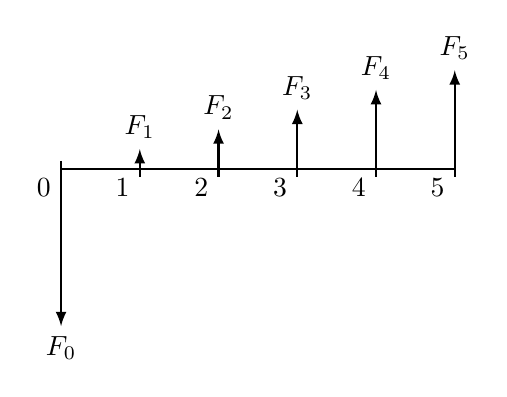
\begin{tikzpicture}[thick]
        \draw (0,0) -- (5,0);
        \foreach \Y [count=\X starting from 0] in {-2, 0.25, 0.5, 0.75, 1, 1.25}
        {\draw[-latex] (\X,0) node[below left]{\X} (\X,{-0.1*sign(\Y)}) -- (\X,\Y)
        node[anchor={sign(\Y)*(-90)}]{$F_{\X}$};}
    \end{tikzpicture}
}
\newline
Where:
\begin{center}
    $F_0$ is P, $F_1 = \$1,000$, $F_2 = \$1,250$, $F_2 = \$1,500$, $F_3 = \$1,750$, and $F_4 = \$2,000$
\end{center}
Firstly, this looks like a linear gradient series. Knowing that all gradient series are made of the base annunity and gradient annunity:
\begin{enumerate}
    \item Setting up composition for annunities:
    \begin{equation*}
        \begin{aligned}
            P = P_1 + P_2,
        \end{aligned}
    \end{equation*}
    Where $P_1$ represents the base annunity and $P_2$ represents the gradient annunity.
    \item Converting base annunity to present worth:
    \begin{equation*}
        \begin{aligned}
            &P_1 = \$1,000(P/A,6\%,5)
            &P_1 = F_1\left(\frac{(1+i)^N-1}{i(1+i)^N}\right) \\
            &P_1 = \$1,000\left(\frac{(1+0.06)^{5}-1}{0.06(1+0.06)^{5}}\right) \\
            &P_1 = \$4,212.36
        \end{aligned}
    \end{equation*}
    \item Converting gradient annunity to present worth:
    \begin{equation*}
        \begin{aligned}
            &P_2 = \$250(P/G,6\%,5) \\
            &P_2 = G\left(\frac{(1+i)^N - iN -1}{i^2(1+i)^N}\right) \\
            &P_2 = 250\left(\frac{(1+0.06)^5 - 0.06*5 -1}{0.06^2(1+0.06)^5}\right) \\
            &P_2 = \$1,983.64
        \end{aligned}
    \end{equation*}
    \item Adding base and gradient annunities together:
    \begin{equation*}
        \begin{aligned}
            &P = P_1 + P_2 \\
            &P = \$4,212.36 + \$1,983.64 \\
            &P = \$6,196 
        \end{aligned}
    \end{equation*}
\end{enumerate}

%SIGNALS END OF THIS HOMEWORK ASSIGNMENT
\newpage

\begin{center}
    \LARGE{\textbf{IND E 250 HW 2}}
\end{center}
\begin{center}
    Homework 2 Problems: \\
    4.2, 4.9, 4.43, 4.46, 4.65, 4.91 (bonus)
\end{center}
\section*{Problem 4.2}
\begin{exrc}
    If your credit card calculates interest based on 13.90\% APR compounded monthly:
    \begin{enumerate}
        \item What are your monthly interest rate and annual effective interest rate?
        \item If your current outstanding balance is \$3,000 and you skip payments for two months, what would be the total balance two months from now?
    \end{enumerate}
\end{exrc}
\subsubsection*{Part 1 - Finding Monthly and Annual Effective Interest Rates}
Converting to monthly interest rate:
\begin{equation*}
    \begin{aligned}
        i = \frac{13.90}{12} = 1.15833\%/month
    \end{aligned}
\end{equation*}
Converting to annual effective interest rate (using compound interest formula):
\begin{equation*}
    \begin{aligned}
        i_a &= (1 + r/CK)^C - 1 \\
        i_a &= (1 + 13.90\%/(1*12))^{12} - 1 \\
        i_a &= 14.82\%
    \end{aligned}
\end{equation*}
\subsubsection*{Part 2 - Finding Future Balance Two Months from Present}
Finding Future Balance with N = 2 months
\begin{equation*}
    \begin{aligned}
        F = \$3,000(F/P,1.15833\%,2) \\
        F = \$3000(1 + 0.0115833)^2 \\
        F = \$3069.90 
    \end{aligned}
\end{equation*}

\section*{Problem 4.9}
\begin{exrc}
    You have three choices in placing your money in a bank account:
    \begin{enumerate}
        \item Bank A pays 9.25\% compounded annually
        \item Bank B pays 9.00\% compounded quarterly
        \item Bank C pays 8.90\% compounded continiously
    \end{enumerate}
    What bank would you open an account with?
\end{exrc}
Solving this via finding the effective annual interest rate - whichever bank account has the highest effective annual interest rate will be the best option for you:
\subsubsection*{Finding Effective Annual Interest Rate for Bank A}
Given:
\begin{equation*}
    \begin{aligned}
        r = 9.25\% \quad K = 1 \quad C = 1
    \end{aligned}
\end{equation*}

\noindent
Finding $i_a$
\begin{equation*}
    \begin{aligned}
        i_a &= (1 + r/CK)^C - 1 \\
        i_a &= (1 + 9.25\%/1)^1 - 1 \\
    \end{aligned}
\end{equation*}

\subsubsection*{Finding Effective Annual Interest Rate for Bank B}
Given:
\begin{equation*}
    \begin{aligned}
        r = 9.00\% \quad K = 4 \quad C = 1
    \end{aligned}
\end{equation*}

\noindent
Finding $i_a$
\begin{equation*}
    \begin{aligned}
        i_a &= (1 + r/CK)^C - 1 \\
        i_a &= (1 + 9.00\%/4)^1 - 1 \\
    \end{aligned}
\end{equation*}
\subsubsection*{Finding Effective Annual Interest Rate for Bank C}
Given:
\begin{equation*}
    \begin{aligned}
        r = 8.90\% \quad K = C = lim_{C \rightarrow \infty} 
    \end{aligned}
\end{equation*}

\noindent
Finding $i_a$
\begin{equation*}
    \begin{aligned}
        i_a = e^{8.90\%} - 1 \\
        i_a = 0.09308 \\
        i_a = 9.308\%
    \end{aligned}
\end{equation*}

\section*{Problem 4.43}
\begin{exrc}
    You burrowed \$12,000 to buy a new car from a bank at an interst rate of 9\% compounded monthly. This loan will be repaid in 48 equal monthly installments over 4 years. Immediately after the 20th payment, you desire to pay the remainder of the loan in a single payment. Compute this lump-sum amount.
\end{exrc}

\section*{Problem 4.65}
\begin{exrc}
    You plan to buy a \$250,000 home with 20\% down payment. The bank you want to finance the loan suggests two options:
    \begin{enumerate}
        \item A 15-year mortgage at 4.25\% APR
        \item A 30-year mortgage at 5.00\% APR
    \end{enumerate}
    What is the difference in monthly payments between these two options?
\end{exrc}

\section*{Problem 4.91}
\begin{exrc}
    The Photo Film Company's bonds have 4 years remaining to maturity. Interest is paid annually, the bonds have a \$1,000 par value, and the coupon interest rate is 8.75\%.
    \begin{enumerate}
        \item What is the yield to maturity at a current market price of \$1,108?
        \item Would you pay \$935 for one of these bonds if you thought the market rate of interest is 9.5\%?
    \end{enumerate}
\end{exrc}



%SIGNALS END OF THIS HOMEWORK ASSIGNMENT
\newpage

\end{document}

